%rubber: module xelatex

\documentclass[]{beamer}

\usepackage{transparents-cours}
\usepackage{graphicx}

\usefonttheme{default}

\subtitle{ASR2 - Système}
\title{Le langage de la machine}

\author{Semestre 2, année 2012-2013}
\institute{
  Département informatique\\
  IUT Bordeaux 1
}
\date{Mars 2013}


\AtBeginPart{
  \frame{\partpage} 
  \frame{
\frametitle{Contenu}
\begin{multicols}{2}
\tableofcontents
    \end{multicols}
  }
}


\begin{document}
\newcommand{\bashlisting}[0]{\lstset{language=bash,numbers=left,numberstyle=\tiny,frame=single}}

\begin{frame}
  \titlepage
\end{frame}


\part{Structure d'un ordinateur}

\section{Éléments}

\begin{frame}
\frametitle{Structure d'un ordinateur}


Un ordinateur comporte
un \emph{processeur},
de la \emph{mémoire}, 
des \emph{dispositifs d'entrée-sortie}.

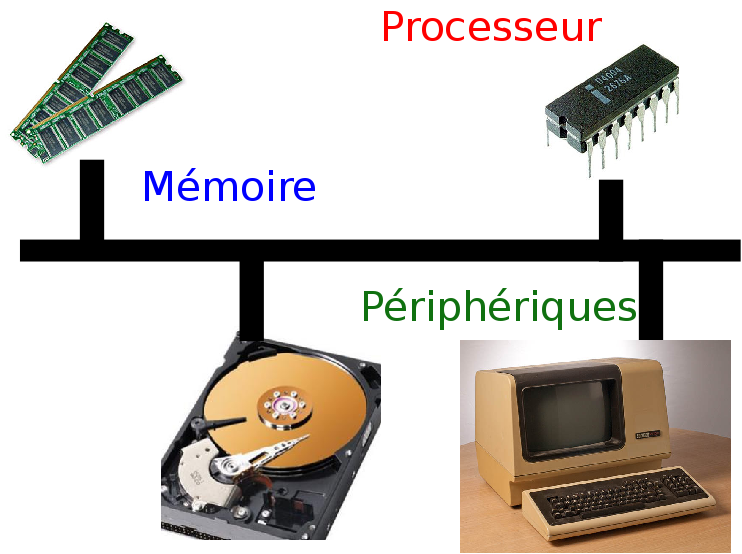
\includegraphics[width=0.8\linewidth]{figures/proc-mem-periph}

\end{frame}

\section{Interaction des éléments}
\begin{frame}
\frametitle{Rôle des éléments}
Ces éléments interagissent : 
\begin{itemize}
\item la \alert{mémoire} contient les \alert{données},
\item le \alert{processeur} exécute les \alert{instructions}
prises dans la mémoire ;
\item ces instructions 
\begin{itemize}
\item effectuent des calculs, 
\item prennent et placent des données 
en mémoire, 
\item les envoient ou les lisent sur les dispositifs d'entrée-sortie
\end{itemize}
\item les \alert{périphériques} assurent
\begin{itemize}
\item le stockage des données à long terme
\item la communication avec l'environnement
\end{itemize}
\end{itemize}

\end{frame}


\section{Le premier ordinateur}
\begin{frame}
\frametitle{SSEM : le premier ordinateur}

\alert{Small-Scale Experimental Machine}, Université de Manchester, 1948

\begin{center}
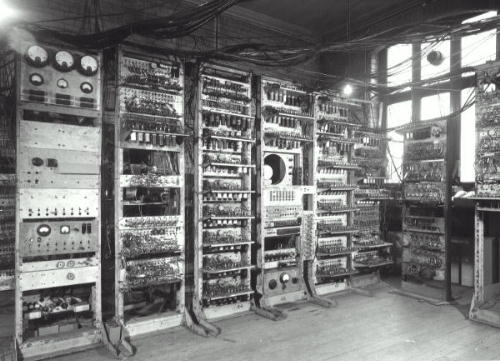
\includegraphics[width=0.6\linewidth]{images/ssem01-2.jpg}
\end{center}
Première machine à \alert{architecture Von Neumann} : \\
\alert{instructions et données} enregistrés {en mémoire}.
\end{frame}

\begin{frame}
\frametitle{SSEM, un calculateur expérimental}
\begin{itemize}
\item \alert{banc de test} pour une nouvelle technologie de mémoire :
  les tubes de Wilkins-Kilburn
\begin{tabular}{lc}
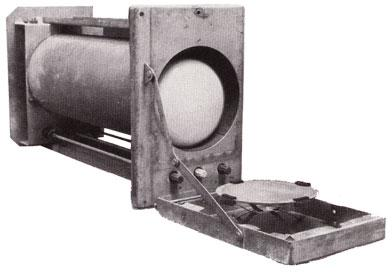
\includegraphics[width=4cm]{images/Williams-tube.jpg} &
 un tube :  32 mots de 32 bits
\end{tabular}
\item \alert{très limité}
\begin{itemize}
\item 330 diodes, 250 pentodes, 
\item un accumulateur 32 bits
\item mémoire de 32 mots
\item 7 opérations, pas d'entrées-sorties
\end{itemize}
\end{itemize}
\end{frame}



\begin{frame}
\frametitle{SSEM : démonstration concluante}

\begin{block}{Démonstration du 21 juin 1948}
\begin{itemize}
\item programme de 17 instructions,
\item 3,5 millions d'instruction en 52 minutes, soit 1,1 KIPS
\end{itemize}
\end{block}


\begin{itemize}
\item Fiabilité des tubes de Williams-Kilburn
  \begin{itemize}
  \item des heures / millions d'opérations sans erreur !
  \item employés dans le premier ordinateur d'IBM (1952)
    \\ IBM 701 : 32 tubes de Williams
    \item ensuite remplacés par les \alert{mémoires à tores de ferrite}
\item et les \alert{mémoires à semi-conducteurs} (fin années 70)
  \end{itemize}
\item \alert{Validation du concept d'ordinateur} : calculateur à programme 
  enregistré en mémoire vive 
\item Début d'une série d'ordinateurs britanniques : \\
  Mark 1, Ferranti
  Mark 1 (1951, premier ordinateur commercialisé), LEO I, II, et III (fabriqués par Lyons), etc.
\end{itemize}
\end{frame}







\section{De nos jours}

\begin{frame}
  \frametitle{De nos jours}
Processeurs beaucoup plus complexes :
plusieurs coeurs,  des lignes de caches,  des coprocesseurs etc.

\alert{Évolution du nombre de transistors par processeur}
\begin{center}
\begin{tabular}{|l|r|l|}
\hline
année &  transistors & processeur\\
\hline
1971 & 2,300 & Intel 4004, premier microprocesseur \\
1978 & 29,000 & Intel 8086, premiers PC \\
1979 & 68,000 & Motorola 68000 \\
1989 &	1,180,000 & Intel 80486 \\
1993 & 	3,100,000 & Pentium \\
1997 & 	9,500,000  & Pentium III \\
2000 & 42,000,000 & Pentium 4 \\
2012 & 1,400,000,000 & Quad-Core + GPU Core i7 \\
2012 & 5,000,000,000  & 62-Core Xeon Phi \\
\hline
\end{tabular}
\end{center}

Source : \url{http://en.wikipedia.org/wiki/Transistor_count}
\end{frame}


\part{Structure d'un processeur}

\section{Principes}

\begin{frame}
  \frametitle{Principes de base d'un processeur}

\begin{multicols}{2}
Dans un processeur il y a 
\begin{itemize}
\item des \alert{registres}  : circuits capables de mémoriser
quelques bits d'information
\item  des \alert{circuits combinatoires} (additionneur, comparateurs, ...),
\item de la \alert{logique séquentielle} pour gérer  le déroulement des différentes phases des instructions
\end{itemize}

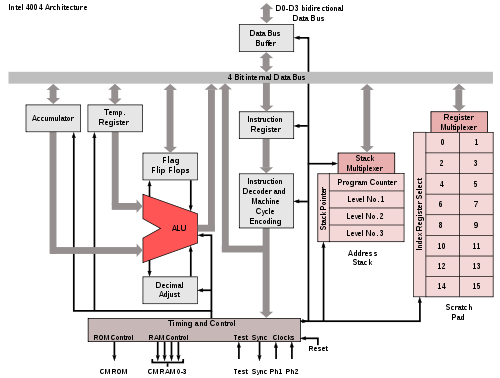
\includegraphics[width=\linewidth]{images/4004_arch.png}
\end{multicols}

\end{frame}

\section{Quelques exemples}

\begin{frame}
  \frametitle{Illustration : architecture du INTEL 4004}
  \begin{center}
  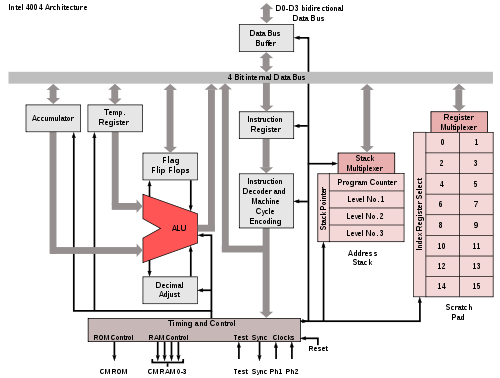
\includegraphics[width=0.8\linewidth]{images/4004_arch.png}
  \end{center}
\end{frame}

\begin{frame}
  \frametitle{Illustration : Architecture ARM, Cortex M3}
  \begin{center}
    
  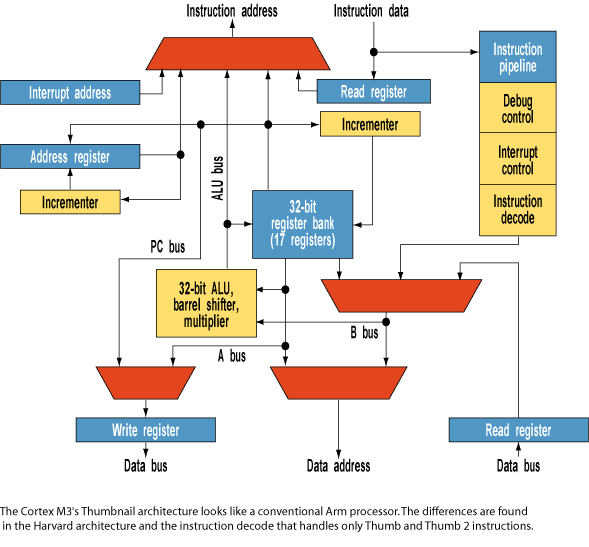
\includegraphics[width=0.6\linewidth]{images/arm-arch.png}
  \end{center}
\end{frame}

\section{Modèle du programmeur}

\begin{frame}
\frametitle{le ``Modèle du programmeur''}
  Le programmeur n'a pas à connaître tous ces détails, seulement 
\begin{itemize}
\item le jeu d'instructions qu'il peut employer

\begin{itemize}
\item les \alert{différents types d'instruction}
\item leur effet sur les registres accessibles
\end{itemize}
\item les registres auquel il a accès
  \begin{itemize}
  \item le \alert{compteur de programme} (adresse de la prochaine instruction)
  \item les \alert{registres} de travail,
\item les \alert{indicateurs de condition}
\item ...
  \end{itemize}
\end{itemize}
\end{frame}




\part{Un processeur fictif}

\section{Exemple pédagogique}
\begin{frame}
\frametitle{Un processeur fictif}  

\structure{Éléments}
\begin{itemize}
\item machine à mots de 16 bits, adresses sur 12 bits
\item 1 accumulateur 16 bits
\item compteur ordinal 12 bits 
\item jeu de 13 instructions sur 16 bits 
  \begin{itemize}
    \item arithmétiques : addition et soustraction 16 bits, complément à 2.
    \item chargement et rangement directs et indirects
      \item saut conditionnel et inconditionnel, appel de sous-programme
      \item ...
  \end{itemize}
\end{itemize}
\end{frame}


\section{Jeu d'instructions}

\begin{frame}
  \frametitle{Format des instructions}

  1 instruction = 16 bits. Format unique : 
\begin{itemize} 
\item \alert{code opération} sur 4 bits (poids forts)
\item \alert{opérande} sur 12 bits
\end{itemize}

\begin{center}
\begin{tabular}{|c|c|}
\hline
code & opérande \\
4 bits & 12 bits \\
\hline
- - - - & - - - - - - - - - - - - \\
\hline
\end{tabular}
\end{center}
\end{frame}

\begin{frame}
  \frametitle{exemple}
Le mot \fbox{\texttt{0011 0000 0110 0100}} (\texttt{Ox3064})
peut représenter une \alert{instruction} 
\begin{itemize}
\item  de code \fbox{\texttt{0011}} = 0x3 
\item d'opérande \fbox{\texttt{0000 0110 0100}} = 0x064 (100 en décimal)
\end{itemize}
\begin{multicols}{2}
qui signifie  ``\emph{ranger le contenu de l'accumulateur dans le mot mémoire d'adresse 100''}
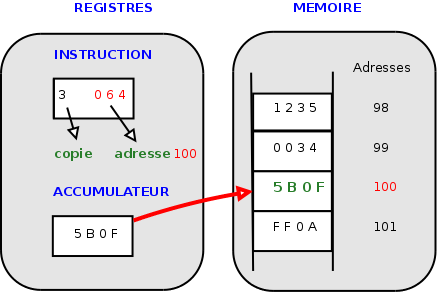
\includegraphics[width=1\linewidth]{figures/store-100.png}
\end{multicols}
\end{frame}

\begin{frame}
  \frametitle{Instruction ou donnée ?}

Le mot 0x3064 représente :
\begin{itemize}
\item une \alert{instruction} (code 3, opérande 100)
\item le \alert{nombre +12388} en binaire complément à 2 
\end{itemize}

La signification d'un mot en mémoire dépend de ce qu'on en fait.
\end{frame}


\begin{frame}[containsverbatim]
  \frametitle{Le jeu d'instructions}


\begin{center}
\footnotesize
\begin{tabular}{|lllll|}
\hline
 & Mnémonique &  Description & Action & \texttt{Cp = } \\
\hline
0 & \texttt{loadi} \emph{imm12} &  \alert{chargement} immédiat &  \verb/Acc = ext(imm12)/ & \verb/Cp + 1/\\
1 & \texttt{load} \emph{adr12} &  chargement direct &  \verb/Acc = M[adr12]/ & \verb/Cp + 1/ \\
2 & \texttt{loadx} \emph{adr12} &  chargement indirect &  \verb/Acc = M[M[adr12]]/& \verb/Cp + 1/ \\
\hline
3 & \texttt{store} \emph{adr12} &  \alert{rangement} direct &  \verb/M[adr12] = Acc/ & \verb/Cp + 1/ \\
4 & \texttt{storex} \emph{adr12} &  rangement indirect &  \verb/M[M[adr12]] = Acc/& \verb/Cp + 1/ \\
\hline
5 & \texttt{add} \emph{adr12} & \alert{addition} & \verb/Acc += M[adr12]/ & \verb/Cp + 1/ \\
6 & \texttt{sub} \emph{adr12} & \alert{soustraction} & \verb/Acc -= M[adr12]/ & \verb/Cp + 1/ \\
\hline
7 & \texttt{jmp} \emph{adr12}  & \alert{saut} inconditionnel & &\verb/adr12/  \\
8 & \texttt{jneg} \emph{adr12}  & saut si négatif & & si \verb/Acc < 0/ \\
  & & & & alors \texttt{adr12} \\
  & & & & sinon \texttt{Cp+1}  \\
9 & \texttt{jzero} \emph{adr12}  & saut si zero & & si \verb/Acc==0/ \\
  & & & & alors \texttt{adr12} \\
  & & & & sinon \texttt{Cp+1}  \\
\hline
A & \texttt{jmpx} \emph{adr12}  & saut indirect & & \verb/M[adr12]/ \\
B & \texttt{call} \emph{adr12}  & \alert{appel} & \verb/M[adr12] = Cp+1/ & \verb/M[adr12]+1 / \\
\hline
C & \texttt{halt 0}  & \alert{arrêt} & &  \\
\hline
\hline
\end{tabular}
\end{center}

\end{frame}

\section{Les classes d'instructions}
\begin{frame}
\frametitle{Les classes d'instructions}


 4  classes :
\begin{block}{Transferts}
pour charger une valeur dans l'accumulateur \\
ou placer le contenu de l'accumulateur en mémoire (\alert{load, store}).
\end{block}

\begin{block}{Arithmétique} addition  et soustraction  (\alert{add, sub})
\end{block}

\begin{block}{Branchements} 
pour continuer à une adresse donnée (\alert{jump, call})
\end{block}
\begin{block}{Divers} 
\alert{halt}
\end{block}

\end{frame}

\section{Programmes}
\begin{frame}
  \frametitle{Programmes}

\begin{itemize}
\item 
\alert{Charger un programme}, c'est remplir la mémoire avec un contenu : instructions et données.

\begin{block}{Exemple de programme)}
  
\texttt{0009 5005 6006 3007 C000 0005 0003 0000}
\end{block}
\item \alert{l'exécution} commence (par convention) au premier mot :
\begin{itemize}
\item le premier mot contient \fbox{0009}, qui correspond à ``loadi 9'' (charger la valeur immédiate 9 dans l'accumulateur)
\item le second mot contient \fbox{5005}, soit ``add 5' (ajouter le mot d'adresse 5 à l'accumulateur)
\item ...
\end{itemize}
\end{itemize}
\end{frame}


\subsection{Utilisation de mnémoniques}
\begin{frame}
\frametitle{Utilisation de mnémoniques}
  
\begin{block}{Exemple de programme}
  
\texttt{0009 5005 6006 3007 C000 0005 0003 0000}
\end{block}

Traduisons les 5 premiers mots en utilisant les \alert{codes mnémoniques} des opérations
\begin{center}
\begin{tabular}{ll|ll}
adresse & contenu & \alert{mnémonique} & opérande \\
\hline
0  & 0009 & loadi & 9 \\
1 & 5005 & add & 5 \\
2 & 6006 & sub & 6 \\
3 &  3007 & store & 7 \\
4 &  C000 & halt & 0 
\end{tabular}
\end{center}


En clair, ce programme charge la valeur 9 dans l'accumulateur, lui ajoute le contenu du
mot d'adresse 5, retranche celui de l'adresse 6 et range le résultat à
l'adresse 7. Et il s'arrête.
\end{frame}

\subsection{Réservation de données}
\begin{frame}
\frametitle{Réservation de mots}

\begin{block}{Exemple de programme}
  
\texttt{0009 5005 6006 3007 C000 0005 0003 0000}
\end{block}

 aux adresses 5, 6, et 7 on trouve les \alert{valeurs} 5,
3 et 0, 
\begin{center}
\begin{tabular}{ll|ll}
adresse & contenu & \alert{directive} & opérande \\
\hline
5  & 0005 & word & 5 \\
6  & 0003 & word & 3 \\
7  & 0000 & word & 0 
\end{tabular}
\end{center}
 
La \emph{directive} \texttt{word} indique la réservation d'un mot mémoire,
avec sa valeur initiale.
\end{frame}


\subsection{Utilisation d'étiquettes}

\begin{frame}[containsverbatim]
  \frametitle{Étiquettes symboliques}

Il est commode de désigner les adresses par des \alert{noms symboliques}, les \alert{étiquettes} :
\begin{multicols}{2}

\begin{lstlisting}[frame=single]
   load  9
   add   5
   sub   6
   store 7
   halt  0

   word  5
   word  3
   word  0
\end{lstlisting}
\break
\begin{lstlisting}[frame=single]
         load  9
         add   premier
         sub   second
         store resultat
         halt  0

premier  word  5
second   word  3
resultat word  0
\end{lstlisting}
\end{multicols}

\end{frame}

\begin{frame}
  \frametitle{Assemblage}

Le programmeur écrit ses programmes en \alert{langage d'assemblage}.\\
 Le code source comporte
\begin{itemize}
\item des instructions
\item des directives de réservation
\item des commentaires
\end{itemize}
qui font apparaître
\begin{itemize}
\item des codes mnémoniques
\item des étiquettes
\end{itemize}
La traduction de ce code source est faite par un \alert{assembleur}.
\end{frame}


\subsection{Conventions d'écriture des sources}
\begin{frame}[containsverbatim]
  \frametitle{Conventions d'écriture}

Sur chaque ligne 
\begin{itemize}
\item 
\alert{l'étiquette est facultative}.
\\ En colonne 1
si elle est présente. \\
Si elle est absente, \alert{la ligne commence un espace} (au moins)
\begin{verbatim}

debut loadi 100     # étiquette et instruction
      sub   truc    # instruction sans étiquette

\end{verbatim}

\item si \alert{l'étiquette est seule}, elle se rapporte au prochain mot
\begin{verbatim}
fin                 # étiquette seule
      halt 0

\end{verbatim}
\end{itemize}
\end{frame}

\part{Programmation}

\section{Codage des expressions et affectations}
\subsection{Rangements, arithmétique, ...}
\begin{frame}
\frametitle{Instructions de base}
Pour commencer : \\
\begin{center}
\begin{tabular}{|rll|}
\hline
chargement & \alert{immédiat} & \alert{loadi valeur} \\
chargement & \alert{direct} & \alert{load adresse} \\
\hline
rangement  &direct & \alert{store adresse} \\
\hline \hline
addition &directe & \alert{add adresse} \\
soustraction &directe & \alert{sub adresse} \\
\hline \hline
arrêt && \alert{halt 0} \\
\hline
\end{tabular}
\end{center}
\alert{Attention ne pas confondre} les opérandes immédiats et directs 
\begin{itemize}
\item \texttt{loadi 100} charge \emph{la constante 100} dans l'accumulateur
\item \texttt{load 100} copie \emph{le mot d'adresse 100} dans l'accumulateur
\end{itemize}
\end{frame}


\subsection{Prise en main du simulateur}

\begin{frame}[containsverbatim]
  \frametitle{Prise en main du simulateur}

{\small
\verb+firefox ~/Bibliotheque/ASR2-systeme/WebSim16/index.html+
}

\alert{Exemple} : traduction de l'affectation ``A = B''

\begin{lstlisting}[frame=single]
    load  B
    store A
    halt 0

A   word 11
B   word 22
\end{lstlisting}

\end{frame}

\begin{frame}
  \frametitle{Utilisation 1/4}

On  tape le programme dans l'\alert{éditeur}

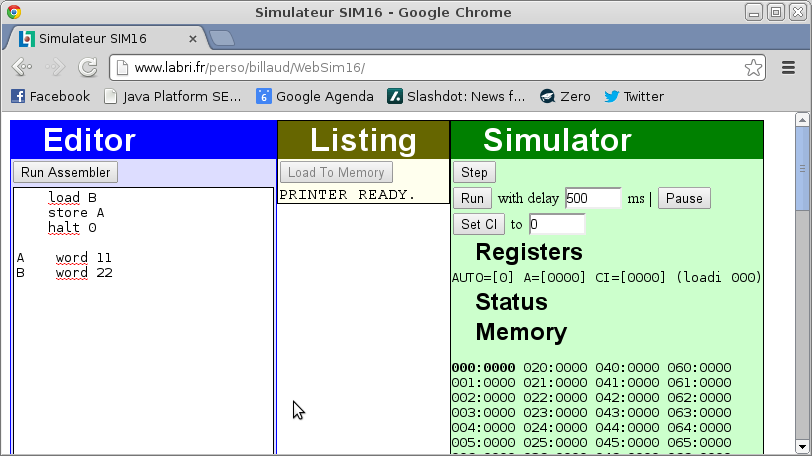
\includegraphics[width=\linewidth]{images/cap1.png}

et on lance l'assembleur...
\end{frame}
\begin{frame}
  \frametitle{Utilisation 2/4}

La fenêtre \alert{Listing} montre un compte-rendu de la traduction.

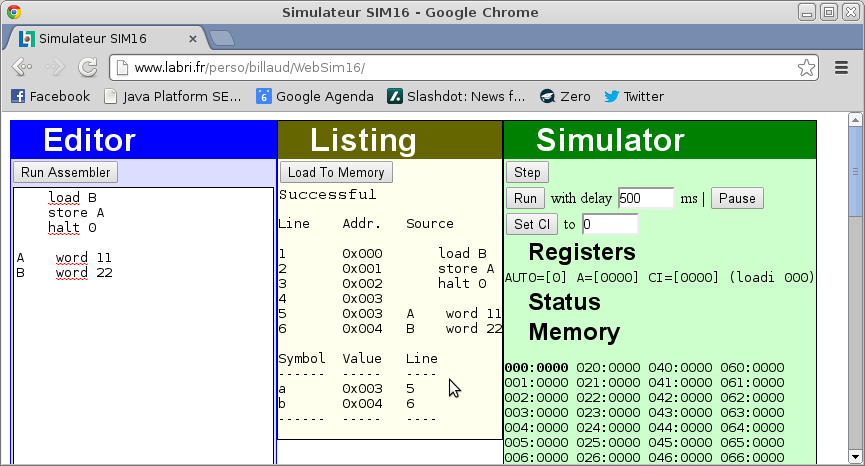
\includegraphics[width=\linewidth]{images/cap2.png}

On charge le code binaire en mémoire
\end{frame}

\begin{frame}
  \frametitle{Utilisation 3/4}

Le programme est chargé dans la fenêtre \alert{Simulator}

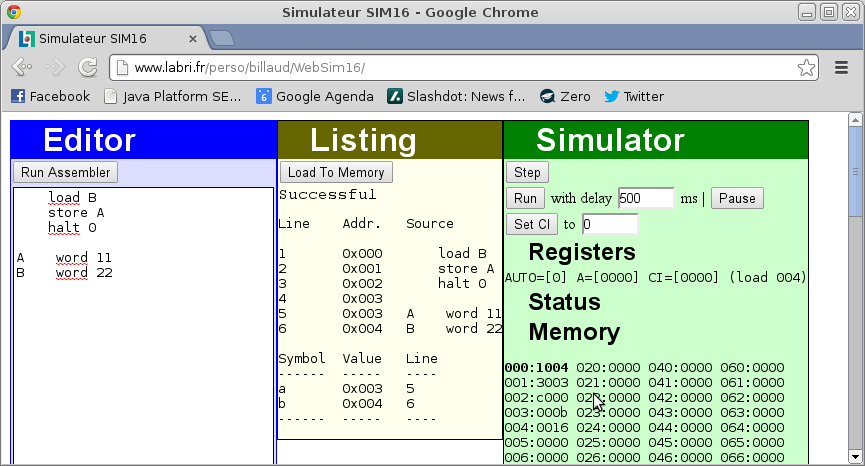
\includegraphics[width=\linewidth]{images/cap3.png}

On peut lancer l'exécution (run)
\end{frame}

\begin{frame}
  \frametitle{Utilisation 4/4}

Le programme se déroule pas à pas

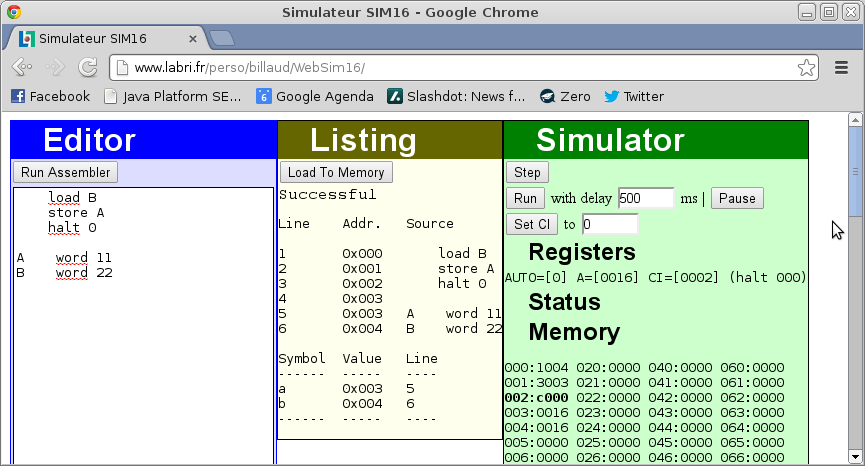
\includegraphics[width=\linewidth]{images/cap4.png}

Et on peut suivre l'évolution du contenu des registres et de la mémoire.

\end{frame}


\subsection{Exercices}
\begin{frame}[containsverbatim]
  \frametitle{Exercices}

\alert{À vous de jouer} : traduisez les affectations 

\begin{itemize}
\item A = A + B 
\item A = A + 1 
\item A = B + C - 1 
\item échange de deux variables  ?
\end{itemize}
\end{frame}

\subsection{Bilan d'étape}
\begin{frame}
\frametitle{Bilan d'étape}
\begin{multicols}{2}
\alert{Bravo !}
\begin{itemize}
\item vous maîtrisez déjà la moitié (presque) des instructions
\item vous savez les employer pour programmer 
  \begin{itemize}
 \item des expressions arithmétiques
\item de affectations
  \end{itemize}
\end{itemize}

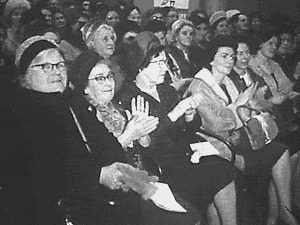
\includegraphics[width=\linewidth]{images/anim/congrats-0}

\end{multicols}

\end{frame}


\section{Décisions et boucles}

\subsection{Saut conditionnels et inconditionnels}

\begin{frame}
\frametitle{Sauts conditionnels et inconditionnel}
Les instructions de saut
\begin{center}
\begin{tabular}{|rll|}
\hline
saut & inconditionnel & \alert{jmp adresse} \\
\hline
saut & si accumulateur nul & \alert{jzero adresse} \\
saut & si accumulateur négatif  & \alert{jneg adresse} \\
\hline
\end{tabular}
\end{center}
qui consultent l'accumulateur et agissent sur le registre ``\alert{compteur de programme}'' (\texttt{Cp}).

Pour les deux \alert{sauts conditionnels}, le déroulement se poursuit
\begin{itemize}
\item à l'adresse indiquée si la condition est vraie (\texttt{Cp = adresse}),
\item en séquence sinon (\texttt{Cp = Cp + 1}).
\end{itemize}
\end{frame}

\subsection{Utilisation}
\begin{frame}[containsverbatim]
  \frametitle{Utilisation}


Instructions rudimentaires, mais suffisantes pour réaliser
\begin{itemize}
\item des alternatives (si-alors, si-alors-sinon, ...)
\item des boucles (tant-que, répéter, ...)
\end{itemize}
\begin{block}{Exemple : calcul de la valeur absolue V d'un nombre X}

Algorithme structuré :
\begin{lstlisting}[frame=single]
   si X < 0
   alors
     |  V = -X
   sinon
     |  V =  X
\end{lstlisting}
\end{block}

\end{frame}

\subsection{Si-alors-sinon}
\begin{frame}[containsverbatim]
  \frametitle{Organigramme 1/4}
  \begin{multicols}{2}
L'algorithme
\begin{lstlisting}[frame=single]
   si X < 0
   alors
     |  V = -X
   sinon
     |  V =  X
\end{lstlisting}
peut être représenté par un
\alert{organigramme}
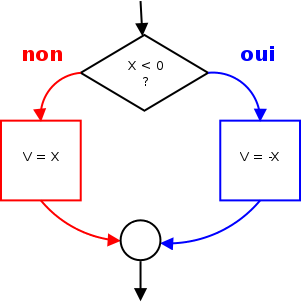
\includegraphics[width=\linewidth]{figures/val-abs-1}    
  \end{multicols}
\end{frame}



\begin{frame}
  \frametitle{Organigramme 2/4}
Faisons maintenant apparaître l'accumulateur :
  \begin{multicols}{2}
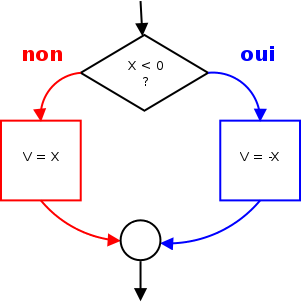
\includegraphics[width=0.9\linewidth]{figures/val-abs-1}
    \break
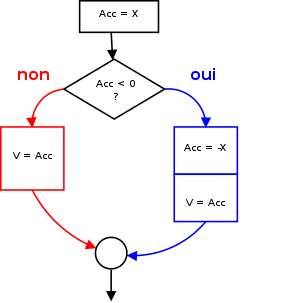
\includegraphics[width=\linewidth]{figures/val-abs-2}    
  \end{multicols}
\end{frame}
\begin{frame}
  \frametitle{Organigramme 3/4 }
L'instruction ``V = Acc'' est la dernière des deux branches, on peut la ``factoriser'' :
  \begin{multicols}{2}
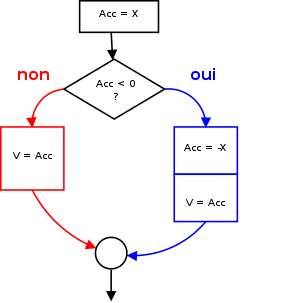
\includegraphics[width=\linewidth]{figures/val-abs-2}    
\break
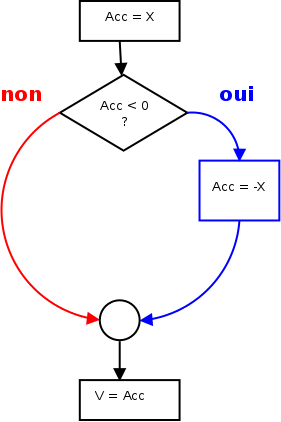
\includegraphics[width=0.8\linewidth]{figures/val-abs-3}    
  \end{multicols}
\end{frame}

\begin{frame}
  \frametitle{Organigramme 4/4}
Si le contenu de l'accumulateur est négatif, l'exécution continue en séquence, il faut alors sauter à la fin.
  \begin{multicols}{2}
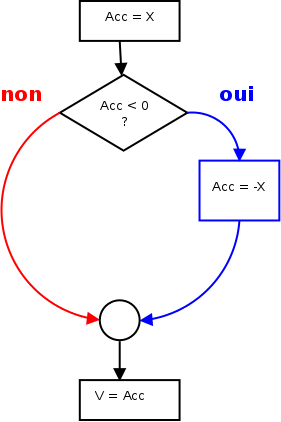
\includegraphics[width=0.7\linewidth]{figures/val-abs-3}    
\break
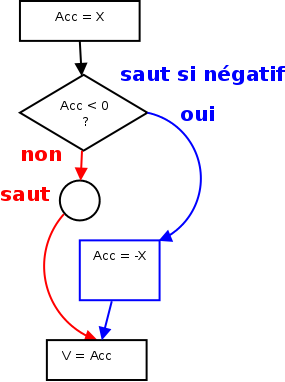
\includegraphics[width=0.8\linewidth]{figures/val-abs-4}    
  \end{multicols}
\end{frame}

\begin{frame}[containsverbatim]
  \frametitle{de l'organigramme au programme}
Il ne reste plus qu'à traduire
  \begin{multicols}{2}
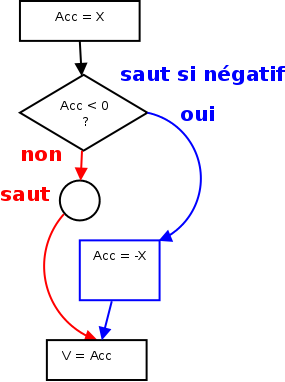
\includegraphics[width=0.8\linewidth]{figures/val-abs-4}    
\break
\begin{lstlisting}[frame=single]
    load X         
    jneg  negatif 
    jmp    fin     
negatif
    loadi  0       
    sub    X
fin
    store  V 
\end{lstlisting}
Ça parait simple...
  \end{multicols}
\end{frame}

\begin{frame}[containsverbatim]
  \frametitle{Commentaires}
Quelques \alert{commentaires} sont indispensables
pour comprendre rapidement la structure du code
\begin{lstlisting}[frame=single]
    load X         # Acc <- X
    jneg  negatif   
    jmp    fin       
                    
negatif            # si Acc < 0 alors
    loadi  0       #       Acc <-  -X
    sub    X       #

fin
    store  V       # V <- Acc 
\end{lstlisting}
\end{frame}


\begin{frame}
\frametitle{Exercices}
\begin{enumerate}
\item \alert{calcul du maximum} M  de deux
nombres A et B


\item \alert{ordonner deux nombres} A et B.

\end{enumerate}

\alert{Indication} : comparer, c'est étudier la différence...
\end{frame}




\section{Faire des boucles}
\subsection{Boucles et organigrammes}
\begin{frame}
\frametitle{Faire des boucles}

Sous forme d'organigramme, deux formes :

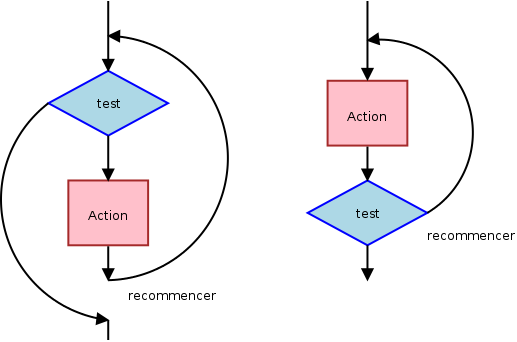
\includegraphics[width=0.8\linewidth]{figures/boucles}    

Avec \alert{test en tête} (boucle ``tant-que'') ou \alert{test en fin} (boucle ``répéter'').
\end{frame}

\begin{frame}[containsverbatim]
\frametitle{Exemple :  la somme des entiers de 1 à N}

\alert{Algorithme}

\begin{lstlisting}[frame=single]
donnée    N nombre, 
résultat  S nombre
variable  K nombre

début
   S = O
   K = 1
   tant que K <= N
    faire
      |   S = S + K
      |   K = K + 1
fin
\end{lstlisting}
\end{frame}


\begin{frame}[containsverbatim]
  \frametitle{Pseudo-instructions}
Séquences d'affectations + sauts conditionnels ou inconditionnels

\begin{multicols}{2}
\small
\alert{Algorithme}
\begin{lstlisting}[frame=single]
début
   S = O
   K = 1
   tant que K <= N
    faire
      |   S = S + K
      |   K = K + 1
fin
\end{lstlisting}
  \break
 \alert{Pseudo-code}
\begin{lstlisting}[frame=single]
    S = 0
    K = 1
BOUCLE
    si K > N aller à SUITE
    S = S + K
    K = K + 1
    aller à BOUCLE

SUITE
    ...
\end{lstlisting}
\end{multicols}
Le test revient à étudier le signe de la différence N-K.
\end{frame}



\begin{frame}[containsverbatim]
\frametitle{Code assembleur}
Le pseudo-code figure en commentaires
\begin{multicols*}{2}
\scriptsize
\begin{lstlisting}[frame=single]
  loadi 0    # S = 0
  store S

  loadi 1    # K = 1
  store K

BOUCLE       # si K > N 
  load  N    
  sub   K
  jneg  SUITE #   aller à suite
    
  load  S    # S = S + K 
  add   K 
  store S

  loadi  1   # K = K + 1
  add    K
  store  K
  jmp   BOUCLE

SUITE
  halt 0

# variables

N  word  5
K  word  0
S  word  0
\end{lstlisting}
\end{multicols*}
\end{frame}

\subsection{Exercices}
\begin{frame}
\frametitle{Exercices sur les boucles}
\begin{block}{Facile}
\begin{enumerate}
\item
programme qui multiplie deux valeurs (additions successives)
\item
programme qui divise deux  valeurs (soustractions successives) et fournit le quotient et le reste.
\end{enumerate}
\end{block}

\begin{block}{À la maison }
\begin{enumerate}
\item programme qui calcule la factorielle d'un nombre.
\item programme qui trouve le plus petit diviseur non 
trivial d'un nombre (plus grand que 1).
\end{enumerate}
\end{block}
\end{frame}


\subsection{Bilan d'étape}
\begin{frame}
\frametitle{Bilan d'étape}
\begin{multicols}{2}
\alert{Bravo !}
\begin{itemize}
\item vous maîtrisez maintenant 6+3 = 9 instructions sur 13
\item vous savez les employer pour écrire des programmes avec  
  \begin{itemize}
\item des affectations
 \item des décisions
\item des boucles
  \end{itemize}
\end{itemize}

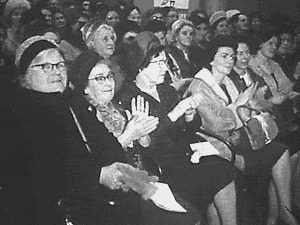
\includegraphics[width=\linewidth]{images/anim/congrats-0}

\end{multicols}
\end{frame}

\section{Tableaux et pointeurs}

\subsection{Adressage indirect}

\begin{frame}[containsverbatim]
  \frametitle{Chargement/rangement indirect}


Deux nouvelles instructions :
\begin{center}
\begin{tabular}{|rll|}
\hline
rangement  &indirect & \alert{loadx adresse} \\
rangement  &indirect & \alert{storex adresse} \\
\hline
\end{tabular}
\end{center}

qui réalisent des chargements /rangements \alert{indirects},
à une adresse indiquée par une variable.
\vspace{1cm}

Elles nous permettront d'utiliser
\begin{itemize}
\item des tableaux
\item des pointeurs
\item ...
\end{itemize}
\end{frame}

\begin{frame}[containsverbatim]
\frametitle{Exemple}

  \begin{multicols*}{2}
\begin{lstlisting}[frame=single]
  loadi   20
  store   100
  loadi   42
  store   101

  loadx   100  
  storex  101  
\end{lstlisting}

copie le mot d'adresse 20 à l'adresse 42, comme le ferait
\begin{lstlisting}[frame=single]
  load   20
  store  42  
\end{lstlisting}

\break
Les mots d'adresse 100 et 101 sont utilisés comme \alert{pointeurs}
vers les données à transférer.

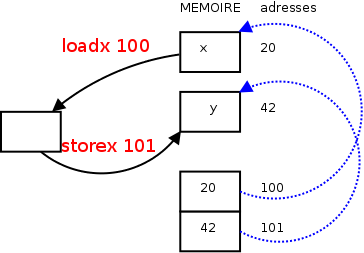
\includegraphics[width=0.8\linewidth]{figures/indirect}

Ils contiennent l'\alert{adresse des données} effectives : les mots d'adresses respectives 20 et 42.


  \end{multicols*}
\end{frame}

\begin{frame}[containsverbatim]
\frametitle{Synthèse : Les types d'opérandes}  


les trois instructions de chargement remplissent l'accumulateur avec
un opérande différent :

\begin{itemize}
\item
\alert{loadi} \emph{constante}  :
la constante figurant dans l'instruction \\ (\alert{opérande immédiat})

\item
\alert{load} \emph{adresse} : 
la donnée située en mémoire, à l'adresse indiquée \\ (\alert{opérande direct})


\item
\alert{loadx} \emph{adresse} :
la donnée pointée par la valeur à l'adresse indiquée \\ (\alert{opérande indirect}).
\end{itemize}

\begin{verbatim}
  loadi valeur             acc =         valeur
  load  adresse            acc =     Mem[adresse]
  loadx adresse            acc = Mem[Mem[adresse]]
\end{verbatim}

\end{frame}

\begin{frame}[containsverbatim]
\frametitle{Illustration}
\begin{itemize}
\item \alert{loadi} (immédiat) charge l'\alert{adresse} d'une variable
(valeur figurant dans l'instruction). \\
Exemple \texttt{002B} = \texttt{loadi 42}
\\ signifie : 
\texttt{Acc = 42}

\item \alert{load} (direct) charge son \alert{contenu} (contenu de la case mémoire).\\
Exemple \texttt{102B} = \texttt{load 42} 
\\ signifie  : 
\verb+Acc = Mem[42]+
\item \alert{loadx} (indirect) charge la donnée qu'elle pointe (\alert{indirection})\\
Exemple \texttt{202B} = \texttt{loadx 42} 
\\ signifie : 
\verb+Acc = Mem[Mem[42]]+

\end{itemize}


\end{frame}





\begin{frame}[containsverbatim]
  \frametitle{Tableaux}
Soit T un tableau (indicé à partir de 0) qui commence à l'adresse 100


  \begin{multicols}{2}
  Pour \alert{accéder au K-ième élément} de T, 
on ajoute 

\begin{itemize}
\item l'\alert{adresse de base} du tableau 100
\item la valeur de \alert{l'indice} K
\end{itemize}
ce qui donne l'adresse de l'élément \verb+T[K]+


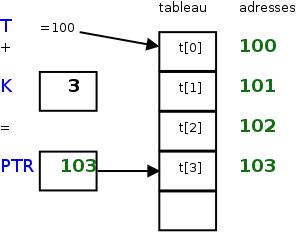
\includegraphics[width=\linewidth]{figures/t100}
  \end{multicols}

Rangée dans un \alert{pointeur} \texttt{PTR}, cette valeur permet
d'accéder à \verb+T[K]+ par \alert{indirection}.
\end{frame}


\begin{frame}[containsverbatim]
\frametitle{Accès à un élément de tableau}
  \begin{multicols}{2}
\small
\begin{lstlisting}[frame=single]

   loadi  T    # adr. de T[0]
   add    K
   store  PTR  # adr. de T[K]

   loadx  PTR  # acc = t[k]
   ...
   storex PTR  # t[k] = acc
   ...
K   word   3
PTR word  0   
T   word  11
    word  22
    ..
\end{lstlisting}

\break
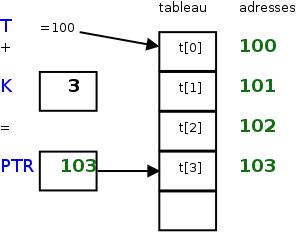
\includegraphics[width=0.8\linewidth]{figures/t100}
  \end{multicols}
\end{frame}



\subsection{Exemple}


\begin{frame}[containsverbatim]
  \frametitle{Exemple : somme des éléments d'un tableau}

\begin{multicols}{2}
\alert{Algorithme en pseudo-code}
\begin{lstlisting}
S = 0
K = 0
tant que K != 10
faire
  |  S = S + T[K]
  |  K = K + 1
\end{lstlisting}
\break
La programmation de la boucle n'a plus de secret pour vous


Il reste à réaliser \verb/ S = S + T[K]/ :
\begin{lstlisting}[frame=single]
    loadi  T
    add    K
    store  PTR

    loadx  PTR
    add    S
    store  S
\end{lstlisting}
\end{multicols}
\end{frame}

\begin{frame}[containsverbatim]
  \frametitle{Exemple : somme des éléments d'un tableau}





\begin{lstlisting}
   loadi 0
   store S
   store K
BOUCLE
   loadi 10       / loadi T
   sub   K       /  add   K
   jzero FIN    /   store PTR
   ........... /    loadx PTR
   loadi 1      \   add   S
   add   K       \  store S
   store K
   jmp   BOUCLE
FIN
   halt  0
\end{lstlisting}

\end{frame}

\subsection{Exercices}

\begin{frame}
  \frametitle{Exercices}

\alert{Simples}
\begin{enumerate}
\item Remplissage d'un tableau avec les entiers de 0 à 9
\item Copie d'un tableau dans un autre
\item Maximum des éléments d'un tableau
\end{enumerate}
\alert{Un peu plus longs...}
\begin{enumerate}
\item Tri par sélection
\item Tri par insertion
\end{enumerate}

\end{frame}


\subsection{Bilan d'étape}
\begin{frame}
\frametitle{Bilan d'étape}
\begin{multicols}{2}
\alert{Bravo !}
\begin{itemize}
\item vous maîtrisez maintenant 11 instructions sur 13
\item et vous savez les employer pour écrire des programmes qui manipulent des tableaux
et des pointeurs.
\item pour finir, nous allons voir l'appel et le retour de sous-programmes.
\end{itemize}

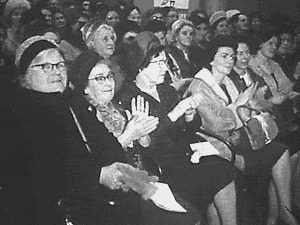
\includegraphics[width=\linewidth]{images/anim/congrats-0}

\end{multicols}
\end{frame}

\section{Sous-programmes}

\subsection{Appel et retour}
\begin{frame}
  \frametitle{Appel et retour}
Les deux dernières instructions :
\begin{center}
\begin{tabular}{|rll|}
\hline
saut  &indirect & \alert{jmpx adresse} \\
rangement  &indirect & \alert{storex adresse} \\
\hline
\end{tabular}
\end{center}
servent à réaliser des sous-programmes :

\begin{itemize}
\item 
\alert{jmpx adresse} fait aller à l'instruction pointée par le contenu de la case mémoire indiqués. \\
Exemple, si le mot
d'adresse 100 contient 25, un \texttt{jmpx 100} fait aller à 25.
\item 
\alert{call} appelle un sous-programme en 
\begin{itemize}
\item sauvegardant l'adresse de l'instruction suivante à l'adresse indiquée
\item poursuivant l'exécution à l'adresse + 1.
\end{itemize}
En effet, un sous-programme commence par un mot réservé, qui
contiendra l'adresse de retour, suivi par le code.

Un exemple ?
\end{itemize}
\end{frame}

\begin{frame}[containsverbatim]
\frametitle{Exemple de sous-programme}
\begin{multicols}{2}

\alert{Séquence d'appel}
\begin{lstlisting}[frame=single]
    loadi   X      
    call    DOUBLER
    store   XX
    ...
\end{lstlisting}
\break
\alert{Le sous programme}\\
 (multiplie l'accumulateur par 2)
\begin{lstlisting}[frame=single]
DOUBLER
  word 0  # adr. retour
  store TMP
  add   TMP
  jmpx  DOUBLER # retour
    ...
\end{lstlisting}
\end{multicols}

Cette manière de faire les appels était utilisée dans quelques
machines (PDP/1, PDP/4, HP 1000....)
\end{frame}


\subsection{Passage de paramètres}

\begin{frame}
\frametitle{Passage de paramètres}

\alert{Le passage de paramètres est une affaire de conventions.}

\alert{Exemple}: la fonction qui calcule le maximum de deux nombres

On peut décider que les paramètres seront fournis
\begin{itemize}
\item  dans deux variables MAXP1 et MAXP2
\item ou au sommet d'une pile d'exécution (tableau en fin de mémoire)
\end{itemize}

et que le résultat sera
\begin{itemize}
\item présent dans l'accumulateur
\item présent dans une variable MAXRESULTAT
\item placé sur la pile
\end{itemize}

Sans parler de passage par référence...
\end{frame}

\subsection{Exercices}
\begin{frame}
\frametitle{Exercices}
Écrivez 
\begin{itemize}
\item un sous-programme de multiplication
\item une fonction factorielle.
\item un sous-programme de division, 
\item un programme qui teste si un nombre est premier.
\item un programme qui remplit un tableau avec les 20 premiers nombres
premiers
\end{itemize}
\end{frame}

\section{Conclusion}

\begin{frame}
\frametitle{Conclusions}
\begin{itemize}
\item 
Un jeu d'instructions très simple suffit à la programmation.
\item
Les langages de programmation ont hérité des concepts des premiers ordinateurs
\begin{itemize}
\item instructions qui modifient les données contenues dans des ``cases'' : c'est la programmation impérative
\item indirection : pointeurs
\end{itemize}
\item
Des notions un peu délicates (comme les tableaux et les pointeurs en C/C++) se comprennent
plus facilement quand on sait ce qui se passe dans la machine. 
\end{itemize}
\end{frame}

\begin{frame}
  \frametitle{La suite}
  \begin{itemize}
\item  La programmation en langage d'assemblage sera étudiée en détail avec
des processeurs modernes (RISC à 3 registres).
\begin{itemize}
\item plus d'instructions 
\item moins fastidieux à utiliser
\end{itemize}
\item
Ce cours continue avec l'initiation au langage C.
  \end{itemize}
\end{frame}



\end{document}

